\documentclass[hyperref={xetex}]{beamer}
\title{Einführung in Matlab und Python - Einheit 7}
\subtitle{Grafik-Handle, Validierung, GUI}
\mode<article>
{
  \usepackage{fullpage}
  \usepackage{pgf}
  \usepackage{hyperref}
  \setjobnamebeamerversion{beamer}
}

\mode<presentation>
{
  %\usetheme{Frankfurt}
 %\usetheme{My}
  \usetheme{Madrid}
  % or ...
%\usecolortheme{seagull}
  %\setbeamercovered{transparent}
  %\setbeamercovered{dynamic}
  % or whatever (possibly just delete it)
}
\usenavigationsymbolstemplate{}
\usefonttheme{structurebold}
\usepackage{multimedia}
\usepackage{tikz}
\usepackage{fontspec,xunicode,xltxtra}
%\usepackage[scaled=.90]{helvet}
% Or whatever. Note that the encoding and the font should match. If T1
% does not look nice, try deleting the line with the fontenc.

\setbeamertemplate{footline}
{
\leavevmode
%\hbox{\begin{beamercolorbox}[wd=.5\paperwidth,ht=2.5ex,dp=1.125ex,
%leftskip=.3cm plus1fill,rightskip=.3cm]{author in head/foot}%
%    \usebeamerfont{author in head/foot}\insertshortauthor
%  \end{beamercolorbox}%
%  \begin{beamercolorbox}[wd=.5\paperwidth,ht=2.5ex,dp=1.125ex,leftskip=.3cm,
%rightskip=.3cm plus1fil]{title in head/foot}%
%    \usebeamerfont{title in head/foot}\insertshorttitle\hfill

\hfill\insertframenumber  \hspace{3pt}

%\inserttotalframenumber
%\hspace*{2ex}
%  \end{beamercolorbox}}%
  \vskip3pt%
}

%\usepackage[english]{babel}
\usepackage[ngerman]{babel}
\selectlanguage{ngerman}

%
% math/symbols
%
\usepackage{amssymb}
\usepackage{amsthm}
% \usepackage{latexsym}
\usepackage{amsmath}
%\usepackage{listings}
\usepackage[framed]{mcode}
%\usepackage{mcode}

\usepackage{mydef}
\usepackage{cmap} % you can search in the pdf for umlauts and ligatures
%\usepackage{colonequals} %corrects the definition-symbols \colonequals (besides others)
\title{Einführung in Matlab}
%
%\subtitle{Disputation} % (optional)

\author{Jochen Schulz}
% - Use the \inst{?} command only if the authors have different
%   affiliation.

\institute{Georg-August Universit\"at G\"ottingen \pgfimage[height=0.5cm]{../figures/unilogo3}}
% - Use the \inst command only if there are several affiliations.
% - Keep it simple, no one is interested in your street address.

\date{\today}

\subject{Einführung in Matlab}
% This is only inserted into the PDF information catalog. Can be left
% out. 



% If you have a file called "university-logo-filename.xxx", where xxx
% is a graphic format that can be processed by latex or pdflatex,
% resp., then you can add a logo as follows:

%\logo{\pgfimage[height=0.5cm]{figures/unilogo3}}


% Delete this, if you do not want the table of contents to pop up at
% the beginning of each subsection:
% \AtBeginSubsection[]
% {
%   \begin{frame}<beamer>
%     \frametitle{Aufbau}
%     \tableofcontents[currentsection,currentsubsection]
%   \end{frame}
% }

\AtBeginSection[]
{
  \begin{frame}<beamer>
    \frametitle{Aufbau}
    \tableofcontents[currentsection,currentsubsection]
  \end{frame}
}


\begin{document}



\begin{document}
\titlepage

%
%figure von ehemals einheit6 rausscueh!
%

\section{Matlab: Grafik-Handle}
\begin{frame}[fragile]\frametitle{Grafik-Objekte}
(engl. \mcode{properties}). 
\begin{itemize}
\item Die Eigenschaften  der Objekte sind  in  sogenannten
{\it handles} gespeichert. Sie liegen dort als \mcode{double}
(Gleitkommazahl) vor.
\item Mit Hilfe dieser Handle können die Eigenschaften 
existierender Grafik-Objekte geändert werden.    
\end{itemize}
\end{frame}
%
% Slide
%
\begin{frame}[fragile]\frametitle{Hierachische Struktur von Grafik-Objekten}
\begin{tabular}{lp{3cm}p{7cm}}
Level 1 & Root & Wurzel-Objekt. Gesamter Darstellungsbereich. Es wird automatisch erzeugt und es gibt nur eins.\\

Level 2 & Figure & Grafik-Fenster. \\

Level 3 & Axes, Uicontrol, Uimenu, Uicontextmenu & Benutzerdefinierte Grafik-Interfaces. 
Die Axes Objekte definieren eine Region im Grafikfenster und ordnen ihre Kinder in
dieser Region an.\\

Level 4 & Image, Line, Text, Surface,... & Die eigentlichen Grafiken. Sie sind Kinder der Axes Objekte.\\
\end{tabular}
\end{frame}
% 
% Slide
%
\begin{frame}[fragile]\frametitle{Umgang mit dem Grafik-Handle}
\begin{itemize}
\item Konstruktion einer Grafik
\begin{matlabin}
x = 0:0.2:2*pi;
plot(x,sin(x))
\end{matlabin}
\item Abfragen und Bedeutung der Handles aller Objekte\\
\begin{columns}[t]
\column{0.38\textwidth}
\begin{matlabin}
h = findobj
\end{matlabin}
\begin{matlab}
h =
         0
    1.0000
  100.0015
    3.0016
\end{matlab}
\column{0.38\textwidth}
\begin{matlabin}
get(h,'type')
\end{matlabin}
\begin{matlab}
ans = 
    'root'
    'figure'
    'axes'
    'line'
\end{matlab} 
\end{columns}
\end{itemize}
\end{frame}
% 
% Slide
%
\begin{frame}[fragile]\frametitle{Umgang mit dem Grafik-Handle }
\begin{itemize}
\item Momentane Einstellung des 'Axes'-Objekts
\begin{matlabin}
set(h(3))
\end{matlabin}
\begin{matlab}
        ActivePositionProperty: [position | {outerposition}]
        ALim
        ALimMode: [ {auto} | manual ]
        AmbientLightColor
               ... 
\end{matlab}
\item Eigenschaften des 'Line'-Objekts
\begin{matlabin}
get(h(4))
\end{matlabin}
\begin{matlab}
        DisplayName: {}
        Color: {}
        LineStyle: {5x1 cell}
        LineWidth: {}
               ... 
\end{matlab}
\end{itemize}
\end{frame}
% 
% Slide
%
\begin{frame}[fragile]\frametitle{Umgang mit dem Grafik-Handle }
\begin{itemize}
\item \"Andern des Markers:
\begin{matlabin}
set(h(4),'Marker','s','MarkerSize',4)
\end{matlabin}
\item \"Andern der Einheiten auf der x-Achse
\begin{matlabin}
set(h(3),'XTick',[0 pi/2 pi 2*pi])
set(h(3),'XtickLabel','0|pi/2|pi|2pi')
\end{matlabin}
\item \mcode{gca}, \mcode{gcf} und \mcode{gco} sind die Handle f\"ur die
  aktuelle {\it Axes}, die aktuelle {\it Figure} und das aktuelle {\it
  Objekt} des 4. Levels.
\begin{columns}[t]
\column{0.5\textwidth}
\begin{matlabin}
set(gcf,'Name','Tolle Abb.')
set(gca,'Fontsize',15) 
\end{matlabin}
\column{0.4\textwidth}
\begin{matlabin}
l = legend('sin(x)');
set(l,'FontSize',20); 
\end{matlabin}
\end{columns}
\end{itemize}
\end{frame}
%
% Slide
%
\begin{frame}[fragile]\frametitle{Hierachie}
\begin{itemize}
\item Informationen zu den zugeordneten Kindern
\begin{matlabin}
a = get(l,'Children'), get(a,'type')
\end{matlabin}
\item Information zu den Eltern
\begin{matlabin}
d = get(l,'Parent'), get(d,'type')
\end{matlabin}
\item \"Andern der Kindeigenschaften
\begin{matlabin}
set(a(3),'Color',[1 0 0])
\end{matlabin}
\end{itemize}
\end{frame}
%
% Slide
%
\begin{frame}[fragile]\frametitle{Beispiel}
\matinput{current_figure.m}
\end{frame}
%
% Slide
%
\begin{frame}[fragile]\frametitle{Umgang mit Objekten}
\begin{itemize}
\item L\"oschen von Objekten:
\begin{matlabin}
delete(handle) 
\end{matlabin}


\item Kopieren von Objekten: 
\begin{matlabin}
copyobj(handle,new_parent) 
\end{matlabin}
H\"angt das Objekt mit Handle \mcode{handle} an andere Eltern
\mcode{new_parent} an.

\item Finden von Objekten mit bestimmten Eigenschaften: 
\begin{matlabin}
findobj(Eigenschaft, Spezifikation)
\end{matlabin}
\end{itemize}
\end{frame}
%
% Slide
%
\begin{frame}[fragile]\frametitle{Defaulteinstellungen}
\begin{itemize}
\item Ansehen der Defaultwerte
\begin{matlabin}
a = get(0,'Factory')
\end{matlabin}
\item \"Andern der Defaultwerte
\begin{matlabin}
set(0,'DefaultLineLineWidth',3)
set(0,'DefaultFigureColor','g')
set(0,'DefaultAxesFontSize',20)
\end{matlabin}
\item Einstellungen gelten immer auch f\"ur alle Kinder und Kindes-Kinder.
\end{itemize}
\end{frame}
%
% Slide
%
\begin{frame}[fragile]\frametitle{Defaulteinstellungen II}
\begin{itemize}
\item L\"oschen der Defaulteinstellung
\begin{matlabin}
set(0,'DefaultAxesFontSize','remove')
\end{matlabin}
\item Die Defaulteinstellungen k\"onnen in der Datei \verb!startup.m!  (Linux/Unix)
   bzw. \verb!matlabroot\toolbox\local! (Windows) abgelegt werden. Sie werden so
  beim Start von MATLAB automatisch eingeladen. 
\item Unter Linux muss die Datei durch den Suchpfad \mcode{path} erreichbar
  sein (oder einfach dort hinlegen: \verb!~/.matlab/startup.m!)
\end{itemize} 
\end{frame}
\begin{frame}[fragile]\frametitle{Ein Beispiel}
\matinput{figure_example.m}
\end{frame}


%
%=============================================================================
%
%
% Slide
%
\section{Grapical User Interface (GUI)}
%
% Slide
%
\begin{frame}[fragile]\frametitle{GUIs in MATLAB}
\begin{itemize}
\item Das Graphical User Interface(GUI) erm\"oglicht das Steuern von Programmen
  mit Hilfe der grafischen Oberfl\"ache. 
\item Programme können von Usern ohne MATLAB-Kenntnisse genutzt werden. 
\item Hilfreich selbst für den Implementierer von numerischen Algorithmen.
\item Steuerung der GUIs durch Grafik-Objekte der Typen
\begin{itemize}
\item \mcode{uimenu}
\item \mcode{uicontextmenu} 
\item \mcode{uicontrol}
\item \mcode{uipanel}
\end{itemize}
(Gleiche Hierachie-Ebene wie \mcode{axes}-Objekte)
\item Grafische Oberfl\"ache zur Erstellung von GUIs:
\begin{matlabin}
guide
\end{matlabin}
 
\end{itemize}
\end{frame}
%
% Slide
%
\begin{frame}[fragile]\frametitle{Vordefinierte GUIs f\"ur Dialogboxen}
\begin{itemize}
\item { \mcode{helpdlg}}: Hilfebox
\item { \mcode{msgbox}}: Eine beliebige Nachricht
\item { \mcode{warndlg}}: Anzeige einer Warnung
\item { \mcode{inputdlg}}: Abfragen einer Gr\"o{\ss}e
\item { \mcode{questdlg}}: Frage
\end{itemize}
\alert{Beispiel:}
\begin{matlabin}
h1 = warndlg('NameFenster','Nachricht')
h2 = errordlg('NameFenster','Nachricht')
ans = questdlg('NameFenster','Nachricht')
ant = inputdlg({'Frage 1','Frage 2','Frage3'},...
  'NameFenster',[1 2 3], {'defAnt1','defAnt2','defAnt3'})
\end{matlabin}
\end{frame}
%
% Slide
%
\begin{frame}[fragile]\frametitle{Grafik-Objekte und GUIs}
\begin{itemize}
\item \alert{ uicontrol}:
Interaktive grafische Objekte, die Aktionen steuern oder bestimmte Optionen setzen.

\item \alert{ uimenu}:
Benutzerdefinierte Men\"uf\"uhrung in einer \mcode{figure} (wird nicht behandelt).

\item \alert{ uicontextmenu}:
Ein Pop-up Men\"u, das erscheint, wenn der Benutzer mit der rechten Maustaste
ein grafisches Objekt anklickt (wird nicht behandelt).
\item \alert{uipanel}:
  Container-Objekt zum Gruppieren von anderen Elementen.
\end{itemize}
\end{frame}
%
% Slide
%
\begin{frame}[fragile]\frametitle{Arten von UiControls}
\centering
\begin{tabular}{ll}
\mcode{'checkbox'} & Wahl von Zust\"anden an/aus \\
\mcode{'edit'}     & Editierbare Texteingabe\\
\mcode{'popup'}    & Auswahl aus Liste bei Anklicken\\ 
\mcode{'listbox'}  & Auswahl aus einer skrollbaren Liste \\
\mcode{'pushbutton'} & Starten eines Events \\
\mcode{'radio'}    & Auswahl einer Option \\
\mcode{'toggle'}  & Wahl des Zustandes: an/aus  \\
\mcode{'slider'}   & Auswahl aus Wertebereich\\
\mcode{'text'}     & Anzeige von Text in einer Box\\
\end{tabular}

\end{frame}
%
% Slide
%
\begin{frame}[fragile]\frametitle{Eigenschaften von UiControls}
\begin{tabular}{lp{0.85\linewidth}}
Style & Art des UiControls \\
\hline
CallBack & Durch Anklicken des Users auszuf\"uhrende Aktion\\
Position & Lage des Uicontrol-Objekts in der \mcode{figure}\newline
          {\scriptsize Eingabe: [links unten Breite H\"ohe]} \newline
          {\scriptsize Einheiten werden durch die \mcode{Units}-Eigenschaft gesteuert.}\\
String   & Textdarstellung. Bei mehreren Optionen durch Eingabe \newline
          {\scriptsize \mcode{string=\{'opt1';'opt2'\}} oder
            \mcode{string='opt1\|opt2'}}\\
Units    & Einheit zur Bestimmung der Lages des UiControls,\newline
          {\scriptsize Werte: \mcode{pixels} (Default), \mcode{centimeters},
          \mcode{normalized} (Werte in $[0,1]$)}\\
Tag      & String zum Auffinden des Objekts durch \mcode{findobj}
\end{tabular}
\end{frame}
%
% Slide
%
\begin{frame}[fragile]\frametitle{Erzeugen von UiControls}
UiControl-Objekte k\"onnen durch \alert{ \mcode{uicontrol}} erzeugt
werden. Aufruf: 
\begin{matlabin}
handle = uicontrol('<eig1>',<wert1>,.., '<eign>',<wertn>)
\end{matlabin}
\alert{Beispiel:}
\begin{matlabin}
u = uicontrol('style','listbox',...
'string','Option1|Option2|Option3',...
'units','centimeters','position',[0 0 3 3])
\end{matlabin} 
\end{frame}

%
% Slide
%
\begin{frame}[fragile]\frametitle{CallBack}
\begin{itemize}
\item Sobald ein GUI-Objekt aktiviert wird, f\"uhrt es MATLAB Code aus. Dies
  wird {\it CallBack} genannt.
\item {\it CallBack} ist eine Eigenschaft von UiControl.
\item Ein GUI-Objekt wird in der Regel durch einen Mausklick oder \"ahnliches
  aktiviert. 
\item CallBack kann eine Funktion oder ein String, der durch \mcode{eval}
  ausf\"uhrbar ist, sein. 
\item Syntax der Callback-Funktion (durch \mcode{guide} erstellt)

\end{itemize}
\end{frame}

%
% Slide
%
\begin{frame}[fragile]\frametitle{CallBack - Syntaxvarianten}
\begin{itemize}
 \item \mcode{function myfile} \\
\mcode{set(h, 'CallBack', 'myfile')}\\
\item \mcode{function myfile(obj, event)} \\
 \mcode{set(h, 'CallBack', @myfile)}\\
\item \mcode{function myfile(obj, event, arg1, arg2)}\\ 
\mcode{set(h, 'CallBack', \{'myfile', 5, 6\})}\\
\item \mcode{function myfile(obj, event, arg1, arg2)}\\ 
\mcode{set(h, 'CallBack', \{@myfile, 5, 6\})}\\
 \item GUIDE
   \begin{matlabin}
function varargout = <objectTag>_Callback(h,ev_data,handles, varargin)}}     
   \end{matlabin}
\begin{itemize}
\item \mcode{objectTag}: ist der Name, der im Tag des Objects gespeichert wird.
\item \mcode{h}: ist der Handle des Objekts, dass die CallBack-Funktion
  aufruft. 
\item \mcode{ev_data}: event-data (normalerweise unnötig).
\item \mcode{handles}: Struktur aller Objekte in der GUI
\item \mcode{varargin}: ist eine  Liste von Argumenten, die an die Funktion
  \"ubergeben wird.  
\end{itemize}
\end{itemize} 
\end{frame}

% 
% Slide
% 
\begin{frame}[fragile]\frametitle{Hinweise}
\begin{itemize}
\item Callback-Funktionen werden immer im Haupt-Workspace
  gestartet. 
\item Mit Hilfe der \mcode{figure}-Eigenschaft \mcode{UserData} k\"onnen Daten an
  das \mcode{figure}-Objekt geh\"angt werden.
\item Der User kann grafische Objekte per Hand schlie{\ss}en. Dies kann zu
  falschen Aufrufen f\"uhren.
\item Man achte darauf, dass man die richtigen Objekte anspricht. Tipp:
  Eigenschaft \mcode{Tag}. 
\item \mcode{hold (<axes_handle>)}: Verhindern, dass Axen-Einstellungen durch nachfolgende plot-Befehle überschrieben werden.
\end{itemize}
\end{frame}
% 
% Slide
%
\begin{frame}[fragile]\frametitle{Beispiel einer GUI}
\begin{center}
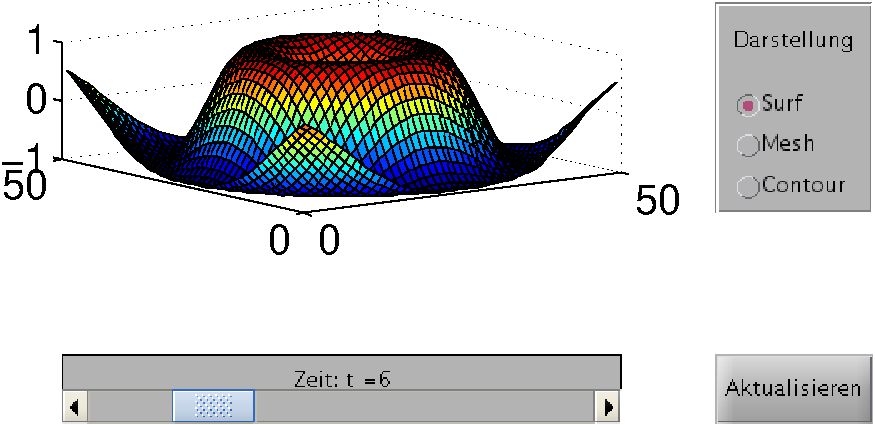
\includegraphics[width=0.9\textwidth]{./figures/gui}
\end{center}
\end{frame}
% 
% Slide
%
\begin{frame}[fragile]\frametitle{bild\_funktion.m}
\begin{matlabin}
function han = bild_funktion()
x = linspace(-1,1,50);
y = linspace(-1,1,50);
t = 0:1:30;
A = erzDaten(x,y,t);
han = erzGUI(A);
end
%------------------- Grafische Oberflaeche erzeugen
function han = erzGUI(A);
delete(findobj('tag','figGUI'));
fig = figure('name','Beispiel GUI','UserData',A,'tag','figGUI');
han.pushbutton = uicontrol(fig,'Parent',fig,'Style',...
  'pushbutton','units','normalized','position',...
  [0.8 0.2 0.15 0.15],'String','Aktualisieren',...
  'Callback','darstGrafik');
han.grafikachse = axes('Position',[0.1 0.5 0.6 0.3],'tag','axesGUI');
han.grafik = surf(A(:,:,1));
\end{matlabin}
\end{frame}
% 
% Slide
%
\begin{frame}[fragile]\frametitle{bild\_funktion.m}
\begin{matlabin}
han.frame1 = uicontrol(fig,'style','frame', 'units',...
  'normalized','position',[0.1 0.2 0.6 0.1]);
han.slider = uicontrol(fig,'style','slider','sliderstep',...
  [0.2 0.2],'min',0,'max',30, 'units','normalized',...
  'position', [0.1 0.2 0.6 0.05],'tag','slider',...
  'Callback','darstGrafik');
han.text1 = uicontrol(fig,'style','text', 'tag',...
  'text1','units','normalized','position', ...
  [0.3 0.25 0.1 0.03],'String','Zeit t = 0');
han.frame2=uibuttongroup('units','normalized','tag','radio',...
  'position',[0.8 0.5 0.15 0.3]);
han.text2=uicontrol(fig,'style','text','parent',han.frame2,...
  'units','normalized','position', [0.1 0.6 0.8 0.3],...
  'String','Darstellung');
\end{matlabin}
\end{frame}
% 
% Slide
%
\begin{frame}[fragile]\frametitle{bild\_funktion.m}
\begin{matlabin}
han.radio1=uicontrol(fig,'style','radio','parent',han.frame2,...
  'tag','r1', 'units','normalized',...
  'position', [0.1 0.45 0.8 0.15],'String','Surf');
han.radio2=uicontrol(fig,'style','radio','parent',han.frame2,...
  'tag','r2','units','normalized',...
  'position', [0.1 0.25 0.8 0.15],'String','Mesh');
han.radio3=uicontrol(fig,'style','radio','parent',han.frame2,...
  'tag','r3','units','normalized',...
  'position', [0.1 0.05 0.8 0.15],'String','Contour');
end
function A = erzDaten(x,y,t)
[X,Y,T] = meshgrid(x,y,t);
A = cos(pi*T.^0.5.*exp(-X.^2-Y.^2));
end
\end{matlabin}
\end{frame}
% 
% Slide
%
\begin{frame}[fragile]\frametitle{darstGrafik.m}
\matinput{darstGrafik.m}
\end{frame}

\section{Validierung}

\begin{frame}{Motivation}
  \begin{block}{Validierung (und Auswertung)}
\begin{itemize}
  \item Validierung von entscheidender Bedeutung für die Numerik
  \item Als Werkzeug dient als wichtiger Teil die Visualisierung 
\end{itemize}
  \end{block}
  \begin{block}{Visualisierung (und Auswertung)}
    \begin{itemize}
  \item Nutze die Intuition und alle Sinne!
      \item Verbindung zur realen Welt
    \end{itemize}
  \end{block}
\end{frame}
%%%%%%%%%%%%%%%%%%%%%%%%%%
\section*{Validierung}
%%%%%%%%%%%%%%%%%%%%%%%%%%
\begin{frame}{Strategien}
  \begin{itemize}
    \item Aufteilung des Problems in möglichst kleine einzelne Module (Funktionen/Klassen) 
    \item Analytische Lösungen numerisch verifizieren
    \item Initial möglichst anschauliche/einfache Probleme berechnen
    \item Benchmarks nutzen: klar definierte Referenzprobleme nutzen
    \item Konsistents-Tests (z.B.):
      \begin{itemize}
        \item  Lösung einer Gleichung Rückwärts nutzen. 
        \item Grössen, Strukturen, Orientierungen und Formate von allen Daten/Matrize/Vektoren prüfen.
        \item Raumzugehörigkeiten prüfen (Falls möglich).
      \end{itemize}
    \item Kondition von Matrizen beachten (Vorkonditionierung, Vermeidung)
    \item Laufzeit-Ausgaben
    \item Dokumentation
    \item Visualisierung nutzen (Intuition!)
  \end{itemize}
\end{frame}


%%%%%%%%%%%%%%%%%%%%%%%%%%%%%%%%%%%%%%
\section*{Visualisierung}
%%%%%%%%%%%%%%%%%%%%%%%%%%%%%%%%%%%%%

\begin{frame}{Subjektive Auswahl von Software/Tools}
  \begin{itemize}
    \item python-like (matplotlib) (script)
    \item VTK, Paraview (gui)
 \item yt (script)
 \item Matlab (gui)
 \item gnuplot (script) 
 \item Visit (gui)
  \end{itemize}
  
\end{frame}

%\begin{frame}{Kategorisierung}
%  \begin{itemize}
%    \item Skalare Funktionen: direkte Einbettung
%    \item Skalare Felder
%      \begin{itemize}
%        \item 1D: Standard x/y-Axenplot
%       \item 2D: Oberfäche (in 3D), Contour, Image
%        \item 3D: Slices, (transparente) Volumina, Isosurface
%      \end{itemize}
 %   \item Vektorwertige Funktionen
 %     \begin{itemize}
 %       \item  Vektorpfeile
 %       \item Tubes
 %       \item Streams
 %     \end{itemize}
 % \end{itemize}
%\end{frame}
%Transparenz: Beispiel? 
%Volumen-beispiele: ?

%**Beispiele:
%heat-equation:analytisches Beispiel? 
%film: heat
%Debug-Ausgaben: heat-equation
%wirbelstrasse (step-35) Beispiel Paraview und gross, glyphs etc.
%(doktorarbeit bzw. huminmd?)


\end{document}
